\documentclass[12pt]{book}
\usepackage[margin=.85in]{geometry} % for MARGIN
\usepackage[many]{tcolorbox}    	% for COLORED BOXES (tikz and xcolor included)


\usepackage{multicol}   
\usepackage{enumerate}
\usepackage[shortlabels]{enumitem}
\usepackage{varwidth}
\usepackage{tasks}
\usepackage[export]{adjustbox}

\usepackage{titleps}
\usepackage{setspace}               % for LINE SPACING
\usepackage[⟨options⟩]{fancyhdr}
\usepackage{enumitem}
\setlist{nosep}
\usepackage{tikz}
\usepackage{pgfplots}
\pgfplotsset{compat=1.5.1}
\usetikzlibrary{datavisualization}
\usetikzlibrary{datavisualization.formats.functions}

\newcommand{\D}{\displaystyle}


\setlength\parindent{0pt}   % killing indentation for all the text
\setstretch{1.3}            % setting line spacing to 1.3
\setlength\columnsep{0.25in} % setting length of column separator
\pagestyle{fancy}           % setting pagestyle to be headings

\usepackage[]{titlesec}

\fancyhead[L]{Math V04 - College Algebra}
\fancyhead[R]{Christina Papazacharioudakis}

\tcbset{
    sharp corners,
    colback = white,
    before skip = 0.2cm,    % add extra space before the box
    after skip = 0.5cm      % add extra space after the box
}                           % setting global options for tcolorbox

    \newtcolorbox{boxR}{
    fontupper = \color{black}, % font color
    boxrule = 1.5pt,
    colframe = black,
    rounded corners,
    arc = 5pt   % corners roundness
}

\definecolor{ballblue}{rgb}{0.13, 0.67, 0.8}

\begin{document}



\begin{comment}
Name: \underline{\hspace{100mm}}
\vspace{20mm}
  \centerline{\Large \textbf{Chapter 2: Equations and Inequalities} } 

{\large
\begin{center}
\begin{varwidth}{\textwidth}
\begin{enumerate}[2.1]
    \item The Regular Coordinate System and Graphs
    \item Linear Equations in One Variable
    \item Models and  Applications (Skipping)
    \item Complex Numbers
    \item Quadratic Equations
    \item Other Types of Equations
    \item Linear Inequalities and Absolute Value Inequalities
\end{enumerate}
\end{varwidth}
\end{center}

}
\newpage  
\end{comment}

{\large \textbf{5.1 Quadratic Functions}}
\\
Recall that in Chapter 2, we looked at a quadratic expression which was an expression of the form $ax^2+bx+c$. We factored them to solve a quadratic equation, $ax^2+bx+c=0$. We now look at quadratic functions, which is a function that is defined as a quadratic: $$ f (x) = ax^2 + bx + c$$

The graph of a quadratic function is a U-shaped curve called a parabola. Let's take a look!
Here is the graph for $f(x)=x^2-2x-3$:
\vspace{3mm}

\centerline{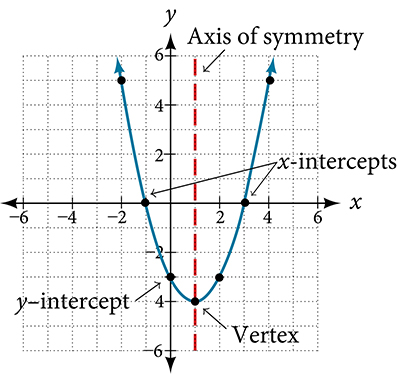
\includegraphics[scale=.6]{Chapter 5/5.1-figure1.jpeg}}




One important feature of the graph is that it has an extreme point, called the \textbf{vertex}. If the parabola opens up, the vertex represents the lowest point on the graph, or the minimum value of the quadratic function. If the parabola opens down, the vertex represents the highest point on the graph, or the maximum value. The graph is also symmetric with a vertical line drawn through the vertex, called the \textbf{axis of symmetry}.

\newpage
  
\underline{\textbf{Example 1 - Identifying the Characteristics of a Porabola}}

   Determine the vertex, axis of symmetry, $x$-intercepts (also called zeros), and  $y$-intercept of the parabola shown. This is the graph for $f(x)=\frac{2}{3}x^2 -4x+7$:

   \centerline{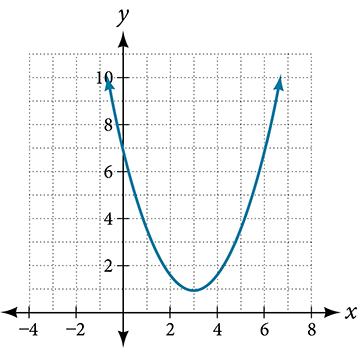
\includegraphics[scale=.5]{Chapter 3/5.1-figure2.jpeg}}

\vspace{80mm}
\begin{boxR}
    \textbf{General Form of a Quadratic Function}
     \vspace{1mm}
     \hline
     \vspace{2mm}
     The \textbf{general form of a quadratic function} is given as
     $$f(x)=ax^2+bx+c$$
     where $a,b$ and $c$ are real numbers and $a \neq 0$. 

      If $a>0$, the parabola opens upward (a smile):
      
      If $a<0$, the parabola opens downward (a frown):

The \textbf{axis of symmetry} can be found using the formula $x= -\frac{b}{2a}$.
 \end{boxR}

 \newpage

 
 

The axis of symmetry comes from the quadratic formula. The $x$-intercepts happen when $y=0$.  That is solving for when $f(x)=0$, or in other words, when $ax^2+bx+c=0$. The quadratic formula tells us that the $x$-intercepts occur when
$$x = \frac{-b \pm \sqrt{b^2-4ac}}{2a} \text{ or } x = -\frac{b}{2a} \pm \frac{\sqrt{b^2-4ac}}{2a} $$
 
 The value of $x$ that is halfway between them is $\D x=\frac{-b}{2a}$, the axis of symmetry. Let's look at an example to demonstrate this: 

{\hspace{-15mm}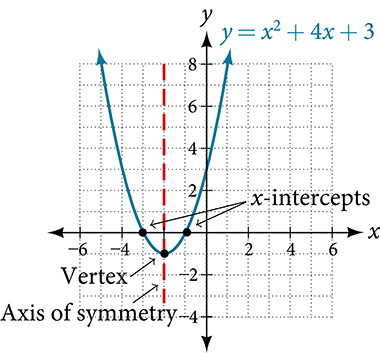
\includegraphics[scale=1.5]{Chapter 5/5.1-figure3.jpeg}}

\vspace{60mm}
How is the vertex and axis of symmetry related? How are they different?
\vspace{25mm}
\begin{boxR}
    The graph of $f(x)=ax^2+bx+c$ has a vertex at $(-\frac{b}{2a}, f(\frac{-b}{2a}))$.
\end{boxR}

\newpage


\begin{boxR}
    The \textbf{vertex form} of a quadratic function is given as 
    $$ f(x)= a(x-h)^2 + k$$
    where $(h,k)$ is the vertex of the parabola. The vertex can also be expressed as $(h, f(h))$
\end{boxR}

As an example, let's identify the vertex in $f(x)=-3(x+2)^2+4$. 




{\hspace{-15mm} 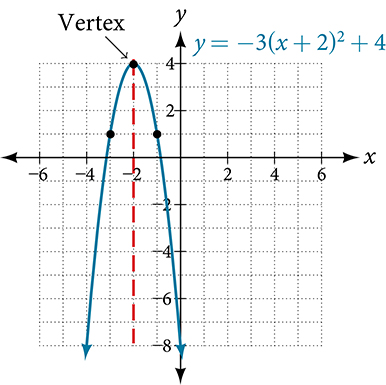
\includegraphics[scale=1.6]{Chapter 5/5.1-figure4.jpeg}}




Notice that the vertex occurs at $(-2, f(-2))$ or more generally, 
$(h, f(h))$.



\vspace{3mm}

\underline{\textbf{Example 3 - Finding the Vertex of a Quadratic Function}}
\\
Find the vertex of the quadratic function $f(x)=2x^2-6x+7$. Once you find the vertex, rewrite the quadratic in vertex form.

\newpage

{\large \textbf{Determining the Maximum and Minimum Values of Quadratic Functions}}

Recall that the highest $y$-value of a function is called the maximum, and the lowest $y$-value of a function is called the minimum. In a quadratic function, these occurs at the vertex. We can see the maximum and minimum values below:

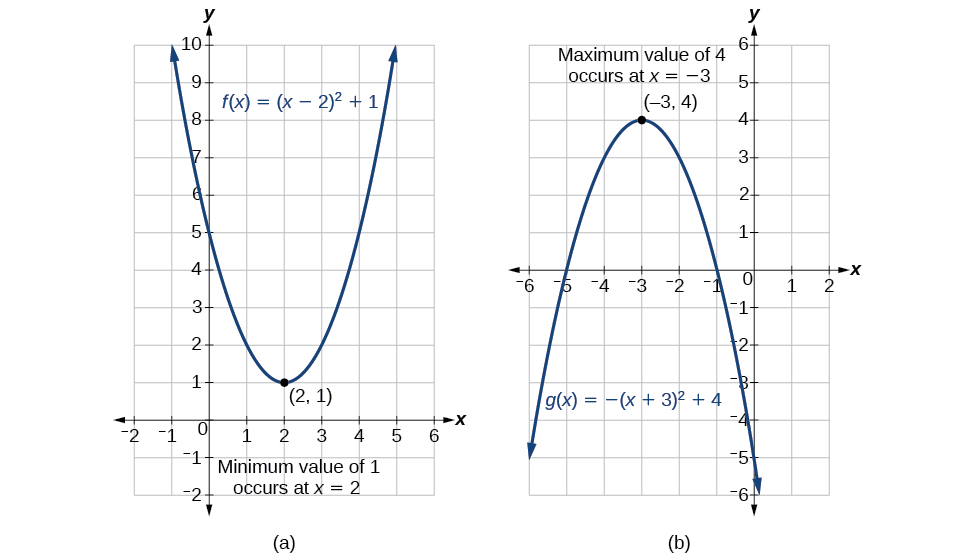
\includegraphics[scale=1]{Chapter 5/5.1-figure5.jpeg}

\newpage

{\large \textbf{Finding the x-Intercepts and y-Intercepts of a Quadratic Function}}

Recall that we find the $y$-intercept of a function by letting $x=0$, and we find the  $x$-intercepts by letting $y=0$. Notice in the figure below that the number of  $x$-intercepts can vary depending upon the location of the graph:

\centerline{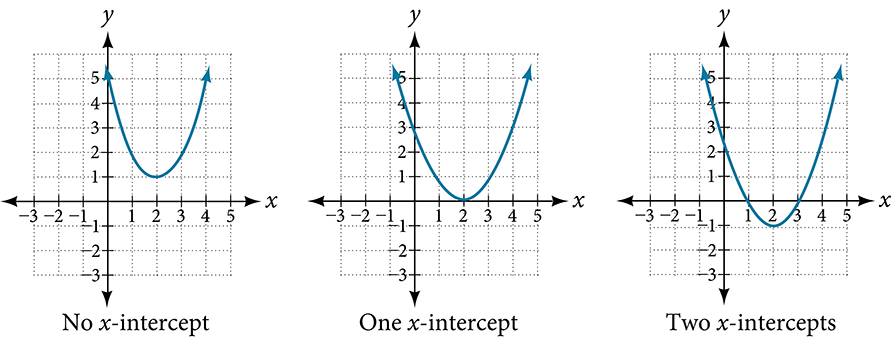
\includegraphics[scale=1.3]{Chapter 5/5.1-figure6.jpeg}}
\vspace{15mm}

The x-intercepts occur when $ax^2+bx+c=0$. The x-values are then $\D x = \frac{-b \pm \sqrt{b^2-4ac}}{2a}$


Recall that the discriminant $b^2-4ac$ told us the nature of these solutions.

$b^2-4ac =0$: 

$b^2-4ac >0$: 

$b^2-4ac < 0$:


\vspace{5mm}

\underline{\textbf{Example 7 - Finding the $y$-Intercepts and $x$-Intercepts of a Parabola}}

Find the $y$-intercepts and $x$-intercepts of the quadratic $f(x)=3x^2+5x-2$. How many $x$ intercepts does it have?


\newpage

\underline{\textbf{Example 8 - Finding the $\mathbf x$-Intercepts of a Parabola}}

Find the $x$-intercepts of the quadratic $f(x)=2x^2+4x-4$. How many $x$ intercepts does it have?







\end{document}


